\documentclass[a4paper]{scrartcl}
\usepackage[utf8]{inputenc}
\usepackage[english]{babel}
\usepackage{graphicx}
\usepackage{lastpage}
\usepackage{pgf}
\usepackage{wrapfig}
\usepackage{fancyvrb}
\usepackage{fancyhdr}
\usepackage{listings}
\pagestyle{fancy}
\usepackage{libertine}
\renewcommand*\familydefault{\sfdefault}  %% Only if the base font of the document is to be sans serif
\usepackage[T1]{fontenc}
\usepackage{courier}
\usepackage[parfill]{parskip}

\graphicspath{ {./images/} }

% Create header and footer
\headheight 27pt
\pagestyle{fancyplain}
\lhead{\footnotesize{Internet Applications, ID1354}}
\chead{\footnotesize{Assignment 3: PHP and Database}}
\rhead{}
\lfoot{}
\cfoot{\thepage\ (\pageref{LastPage})}
\rfoot{}

% Create title page
\title{Assignment 3: PHP \& Database}
\subtitle{Internet Applications, ID1354}
\author{Emil Tullstedt [emiltu@kth.se]}
\date{2014-10-05}

\lstset{
	basicstyle=\footnotesize\ttfamily, 
	numbers=left,
	breaklines=true,
	frame=l,
	keywordstyle=\bfseries\color{blue!40!black},
    stringstyle=\color{red},
    commentstyle=\color{green},
    identifierstyle=\color{black},
    showstringspaces=false
}

\begin{document}

\maketitle

\section{Introduction}

The third assignment for ID1354's purpose is to add server-side scripting functionality to the previously JavaScript and HTML-only site:

\begin{itemize}
\item Enable for user log in, log out and sign up
\item Develop the comment field into a non-volatile version
\end{itemize}

\section{Method}

\subsection{PHP, Flight}

PHP is one of the most widely used web software programming languages. It's usage is because of it's forgiving style, being a loosely and dynamically typed unsafe language with a specialized focus on the web, wielding a zillion built-in functions for practically any need you could imagine when developing a website.

Without further discussing the qualities and flaws of PHP, there are a few key points to be aware of when developing in PHP, namely:

\begin{itemize}
\item PHP isn't inherently built to be object-oriented. In later versions of PHP, the PHP crew have done a good job at supporting classes and objects, but it's still not a de facto standard for PHP to write code in an object oriented fashion
\item PHP is built without using templating, so it's up to the discretion of the programmer to ensure that the views, helpers, models and controllers are adequately separated.
\end{itemize}

With this in mind, it is a good idea to import a framework to work with PHP. The minimal framework Flight is a good example of the best parts of PHP - the feeling of getting stuff done, albeit in a quick'n'dirty way.

\subsection{PostgreSQL}

The database is important, because a good database design will support the developer rather than make the developer feel trapped in a corner. One of the most widely used open source relational database out there is the PostgreSQL database.

There's not much to be said about the database for such a simple project, but there's a few SQL-features that is useful and easily bypassed if you're just seeing SQL as "the place where I store data" rather than as a complex system of data management. Things that are good to be aware of is the \textit{postgres crypto}-module which  allows for easily implemented and cryptographically secure hashing of passwords in the database rather than in the server-side scripting. It may also be useful to be aware of both the ability to write functions that'll enable more sensible SQL-queries and views that can combine data from multiple tables into one.

\section{Result}
\label{sec:results}

The addition of PHP to the site was done gradually, beginning with defining the PostgreSQL layout.

\subsection{Database Schema}

\begin{figure}[!h]
  \begin{center}
    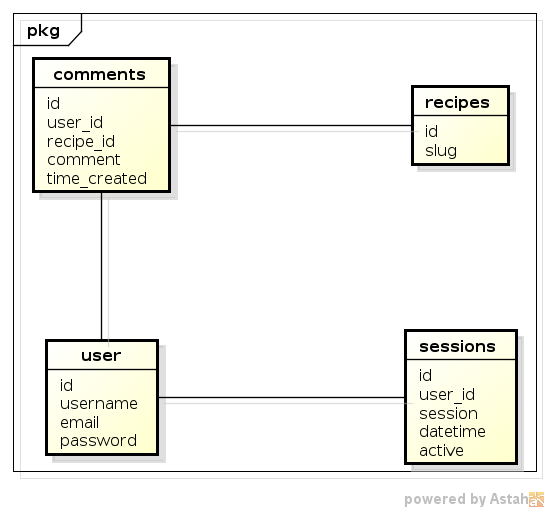
\includegraphics[scale=0.6]{database_schema.png}
    \caption{Database Schema for the database}
    \label{fig:schema}
  \end{center}
\end{figure}

The key behind all persistent storage is the database, and as there may be neither login, registration, comments or any other persistent storage-dependent programming without the database, the first thing to do when developing a server-side, database-driven, website is to create a simple schema over the layout of the database. This is easily done by first making a super-simple graph with the properties of the database, as seen in Fig. \ref{fig:schema}.

The graph then needs to be transferred to an actual schema. In the example from Fig. \ref{fig:schema}, we can see that the user and the recipes-tables doesn't contain any foreign key (this can of course be made even more clearly by using a standardized notation rather than relying on descriptive names) thus we only need to create them as we find fit. We do this in PostgreSQL by declaring:

\begin{lstlisting}[language=SQL]
CREATE TABLE users
(
	id serial PRIMARY KEY,
	username varchar(100) UNIQUE NOT NULL,
	email varchar(255),
	password text
);

CREATE TABLE recipes
(
	id serial PRIMARY KEY,
	slug varchar(100) UNIQUE NOT NULL
);

INSERT INTO recipes(slug) VALUES ('meatballs');
INSERT INTO recipes(slug) VALUES ('pancakes');
\end{lstlisting}

The tables for comments and sessions contains \texttt{user\_id} and the comments table contains \texttt{recipe\_id} as well. These are supposed to be \emph{foreign keys} which means that they are referring to a key which is present in another table. The foreign keys adds a so called constraint onto the database that makes it possible to make it impossible to delete a recipe without also deleting it's comments for example, which is very useful as it makes the database less prone to contain orphans which leads to annoying bugs.

The following SQL-code is used for the comments and sessions table:
\begin{lstlisting}[language=SQL]
CREATE TABLE sessions
(
	id serial PRIMARY KEY,
	user_id integer NOT NULL,
	session text NOT NULL,
	datetime timestamp with time zone DEFAULT now(),
	active boolean DEFAULT TRUE,
	CONSTRAINT sessions_fk1 FOREIGN KEY (user_id)
	REFERENCES users (id)
);

CREATE TABLE comments
(
	id serial PRIMARY KEY,
	user_id integer,
	recipe_id integer NOT NULL,
	comment text NOT NULL,
	time_created timestamp with time zone DEFAULT now(),
	CONSTRAINT comment_fk1 FOREIGN KEY (user_id)
	REFERENCES users (id),
	CONSTRAINT comment_fk2 FOREIGN KEY (recipe_id)
	REFERENCES recipes (id)
);
\end{lstlisting}

\begin{figure}[!h]
  \begin{center}
    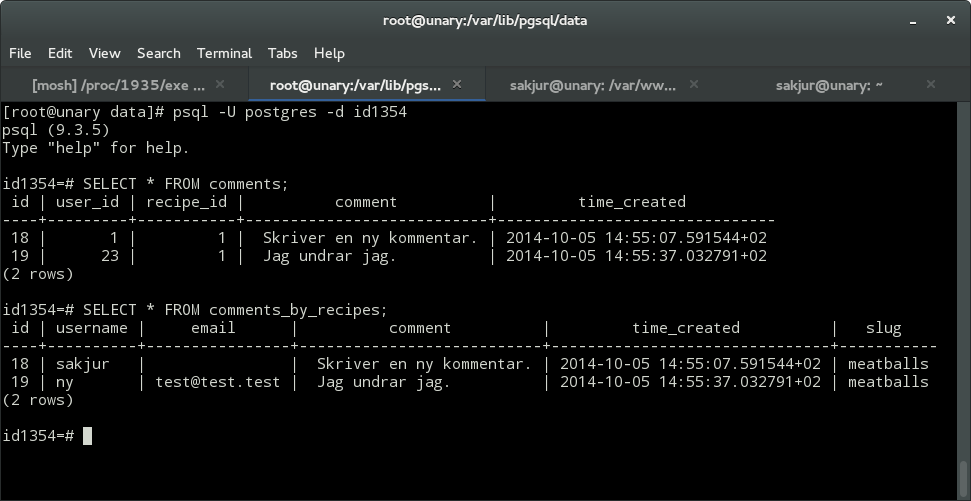
\includegraphics[scale=0.3]{select.png}
    \caption{Sample Query demonstrating Views}
    \label{fig:samquery}
  \end{center}
\end{figure}

If we now add a few rows and then have a look at the rows in the table \texttt{comments} we notice how the table stores the integer identifiers for the user and the recipe relation as in Fig. \ref{fig:samquery}. To make it easier to fetch the comments with the human friendly \texttt{username} and \texttt{slug} identifiers for the user and the recipe respectively we create a view. The view for more sensible output for comments is created as

\begin{lstlisting}[language=SQL]
CREATE VIEW comments_by_recipes AS
	SELECT comments.id, username, email, comment, time_created, recipes.slug
		FROM users, comments, recipes
		WHERE comments.recipe_id = recipes.id AND users.id = comments.user_id;
\end{lstlisting}

This makes it possible to, as demonstrated in Fig. \ref{fig:samquery} execute the query \texttt{SELECT * FROM comments\_by\_recipes;} to get a more useful result.

After having added the view, we are almost done with the database schema, but we want to add two \textit{functions} as well, to make it easier to login and create users. This is a fair bit over-course, but the SQL query for this looks like 

\begin{lstlisting}[language=SQL]
CREATE EXTENSION IF NOT EXISTS pgcrypto;

CREATE OR REPLACE FUNCTION login(_username text, _pwd text, OUT _session_key text)
	RETURNS text
AS $$
	DECLARE
		_userid integer;
	BEGIN
		_session_key := (SELECT crypt(_username || current_timestamp,
			gen_salt('bf')) FROM users
		WHERE users.username = _username
			AND password = crypt(_pwd, users.password));
		_userid := (SELECT id FROM users WHERE username = _username);
		INSERT INTO sessions (user_id, session) VALUES (_userid, _session_key);
	END;
$$ LANGUAGE plpgsql;

CREATE OR REPLACE FUNCTION add_user(INOUT _userid text, _pwd text, INOUT _email text)
	RETURNS record
AS $$
	BEGIN
		INSERT INTO users(username, password, email)
		VALUES (_userid, crypt(_pwd, gen_salt('bf')), _email);
	END;
$$ LANGUAGE plpgsql;
\end{lstlisting}

These functions are largely inspired by code available from the presentation to a talk by Magnus Hagander\footnote{http://www.hagander.net/talks/Secure\%20password\%20storage.pdf}, but modified to fit the specific application.

The code takes care of the salting, verification and hash storage of the password using the \textit{Blowfish}-hashing function.

\subsection{Routing \& the Controller}

The controller is where the Flight-framework is extensively employed and takes care of incoming HTTP-connections from the user.

As most of the content is static, the controller mostly routes the user to the view, with a few notable exceptions. The controller can be seen in it's entirety below:
\lstinputlisting[language=PHP]{../src/index.php}

There is no logic stored within the controller, so it's fairly uninteresting. Where there is need for interactivity, for example where the comments are fetched from the server, the controller does this job and passes it to the view using the Flight-globals. The views doesn't connect to the models directly, and the models aren't aware of either flight nor the views.

\subsection{Models}

There are three models employed in the application, one for handling of databases and then two models that connect to the database handler and presents the database queries in a sensible form to the controller to pass on to the views.

The database model is well encapsulated and works as a solid object which cannot be used to execute arbitrary code, which means there are no SQL queries in the PHP-application outside of this file.

\subsubsection{Database-model}
\label{subsub:databasemodel}
\lstinputlisting[language=PHP]{../src/models/database.php}

The sessions model connects to the database model and presents a few functions to the user of the model that will enable the user to check if a session is valid, create a new session, create a new user and delete a session.

\subsubsection{Session-model}
\label{subsub:sessionmodel}
\lstinputlisting[language=PHP]{../src/models/sessions.php}

The comments model is similar to the sessions model in the sense that it presents useful functions to the user, but unlike the session the comments model is for adding and editing comments. Notable is that the comments-model and the comments-helper are two vastly different and independent structures, where neither are aware of the other's existence.

\subsubsection{Comments-model}
\label{subsub:commentmodel}
\lstinputlisting[language=PHP]{../src/models/comments.php}

\newpage
\subsection{Helpers}

As the views needs the functionality that comes with server-side scripting, but shouldn't connect directly to the models to get the logic and shouldn't contain any logic in themselves, especially when this logic is shared between different views, there are view helpers that contain functions which sole purpose is to make dynamic data presentable for the view.

The helpers are for menus, comments and the header, where the header helper is simply just containing a function to echo the correct JavaScript and CSS imports and is of little interest, the menu helper is slightly more advanced containing both a generator for the menu that employs a new object \texttt{NavLink} that can generate a navigation with dropdown menus in a way that makes sense programmatically. This helper can be seen in subsection \ref{subsub:Menu-helper}.

\subsubsection{Menu-helper}
\label{subsub:Menu-helper}
\lstinputlisting[language=PHP]{../src/views/helpers/menu.php}

\subsubsection{Comments-helper}
\label{subsub:commentshelper}
The most important helper is the comments helper which formats the comments correctly and ensures that only signed in users are presented with the option to add comments and edit (their own) comments. This is further enforced in the comments model, but the comments helper makes sure not to create any issues for the user.

\lstinputlisting[language=PHP]{../src/views/helpers/comments.php}

\section{View}

\begin{figure}[!h]
  \begin{center}
    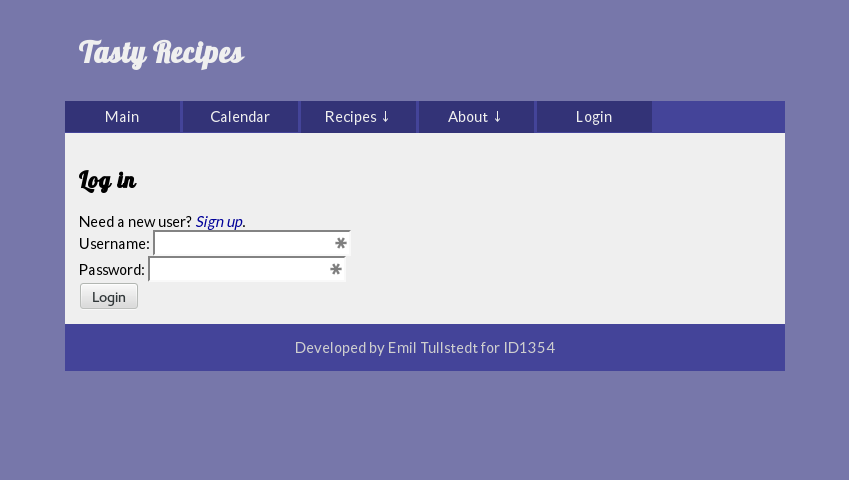
\includegraphics[scale=0.3]{login.png}
    \caption{The new login page}
    \label{fig:login}
  \end{center}
\end{figure}


The views is only slightly changed from the previous seminar in terms of functionality, where the most prominent change is the addition of a login-screen as seen in \ref{fig:login}. The login screen's source further shows how the helpers are called from within the source of the views.

\lstinputlisting[language=PHP]{../src/views/login.php}

The second notable change is in the comment field, which is powered by a server-side backend now. 

The simple addition of the code
\begin{lstlisting}
 $.post('/new_comment', { r: recipe_name, c: comment});
\end{lstlisting}
within the JavaScript that handles the submit button on the comments page made this change possible. This makes it possible to add a comment without reloading the page, as the comment is instantly added as a visual queue to the user and then sent to the server for processing. The obvious disadvantage is that if a submission goes awry, the user will not notice until they've reloaded the page.


\begin{figure}[!h]
  \begin{center}
    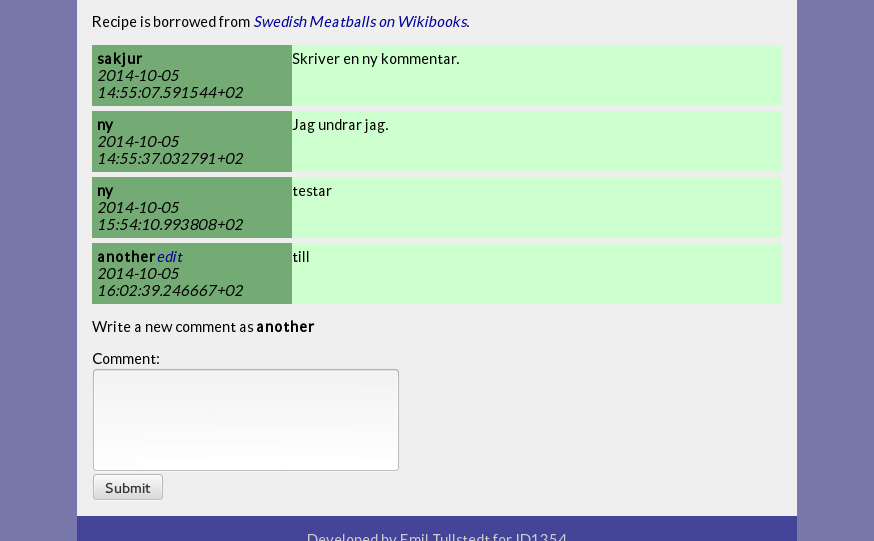
\includegraphics[scale=0.3]{comments.png}
    \caption{The new comments page, for logged in users}
    \label{fig:comments}
  \end{center}
\end{figure}

\begin{figure}[!h]
  \begin{center}
    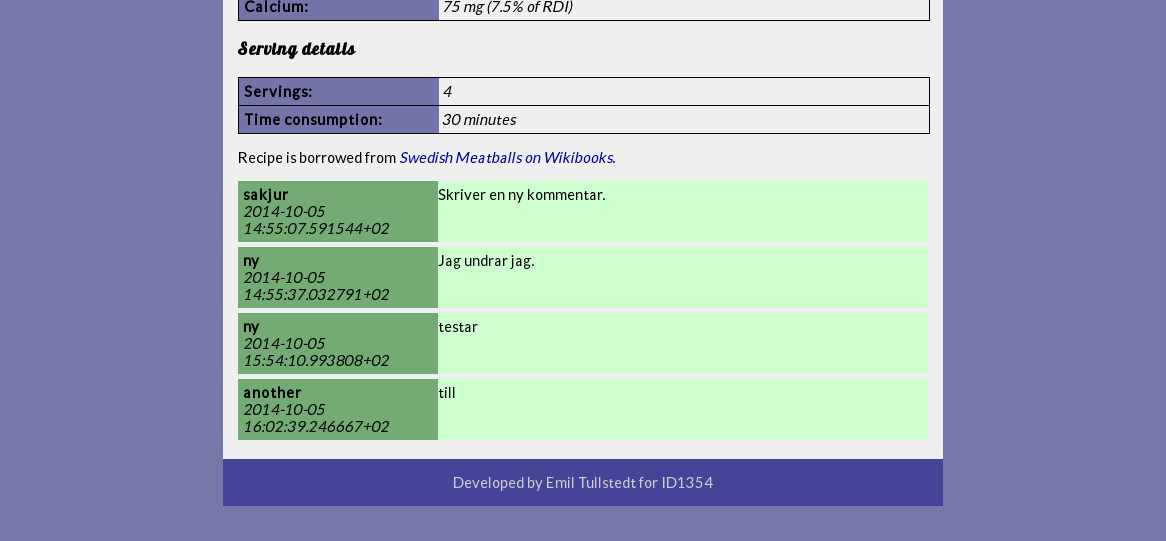
\includegraphics[scale=0.3]{comments_no_login.png}
    \caption{The new comments page, for guests}
    \label{fig:commentsguest}
  \end{center}
\end{figure}

Furthermore, the fields for username and e-mail has been deprecated from the comment page as seen in Fig. \ref{fig:comments}. The entire submission field is removed for the guests as seen in Fig. \ref{fig:commentsguest}.

\newpage
\section{Discussion}

Using PHP, PostgreSQL and Flight provides a powerful toolkit that I would prefer to have had access to from the very beginning. Adding server side code onto a page after adding the JavaScript felt wrong and harsh, as the JavaScript is only supposed to improve the user experience. There are several known design issues with my code, and this is mostly because of lack of time\footnote{as always}. The way PHP is parsed in a "top-down" sense makes it very hard to confirm that you've managed to separate the different parts according to an MVC pattern, and the classes in PHP is sadly not well documented and hard to use extensively. I think that my solution to this problem was as elegant as my level of PHP expertise would allow me.

Would writing this application in Python, Ruby, Erlang or C be easier? Probably not, it would probably take a bit more time, but be more easily maintainable in the end. 

\end{document}
